\documentclass[12pt, preprint]{aastex}
%\usepackage{bm, graphicx, subfigure, amsmath, morefloats}
\bibliographystyle{apj}
\usepackage{float, bm, graphicx, subfigure, amsmath, morefloats}
\usepackage{color}
%\usepackage{caption}
%\usepackage{subcaption}
\usepackage[caption=false]{subfig}

% naming macros
\newcommand{\tc}{\textsl{The~Cannon}} 
\newcommand{\cannon}{\textsl{Cannon}} 
\newcommand{\apogee}{APOGEE}
%\newcommand{\apogee}{\textsl{APOGEE}} 
\newcommand{\aspcap}{ASPCAP}
%\newcommand{\aspcap}{\textsl{ASPCAP}}
\newcommand{\lamost}{LAMOST}
%\newcommand{\lamost}{\textsl{LAMOST}}
\newcommand{\apokasc}{APOKASC}
\newcommand{\segue}{SEGUE}
%\newcommand{\segue}{\textsl{SEGUE}}
\newcommand{\rave}{RAVE}
%\newcommand{\rave}{\textsl{RAVE}}
\newcommand{\galah}{GALAH}
%\newcommand{\galah}{\textsl{GALAH}}
\newcommand{\gaiaeso}{Gaia-ESO}
\newcommand{\gaia}{Gaia}
\newcommand{\kepler}{\textsl{Kepler}}
\newcommand{\ulyss}{\textsl{ULySS}}

% math and symbol macros
\newcommand{\set}[1]{\bm{#1}}
\newcommand{\teff}{\mbox{$\rm T_{eff}$}}
\newcommand{\logg}{\mbox{$\rm \log g$}}
\newcommand{\mh}{\mbox{$\rm [M/H]$}}
\newcommand{\feh}{\mbox{$\rm [Fe/H]$}}
\newcommand{\afe}{\mbox{$\rm [\alpha/Fe]$}}
\newcommand{\alpham}{\mbox{$\rm [\alpha/M]$}}
\newcommand{\cm}{\mbox{$\rm [C/M]$}}
\newcommand{\carbon}{\mbox{$\rm [C/H]$}}
\newcommand{\cn}{\mbox{$\rm [C/N]$}}
\newcommand{\cfe}{\mbox{$\rm [C/Fe]$}}
\newcommand{\nitrogen}{\mbox{$\rm [N/H]$}}
\newcommand{\nfe}{\mbox{$\rm [N/Fe]$}}
\newcommand{\nm}{\mbox{$\rm [N/M]$}}
\newcommand{\ak}{\mbox{$\rm A_k$}}
\newcommand{\starlabel}{\ell}
\newcommand{\starlabelvec}{\set{\starlabel}}
\newcommand{\given}{\,|\,}
\newcommand{\angstrom}{\mbox{\AA}}

\newcommand{\nabundances}{15}
\newcommand{\ntrobj}{9173}
\newcommand{\ntestobj}{275,193}
\newcommand{\snr}{S/N}
\newcommand{\afebias}{-0.00765}
\newcommand{\afescat}{0.0506}
\newcommand{\tefferr}{4.4 K}
\newcommand{\nbssamples}{20}
\newcommand{\loggerr}{0.012 dex}
\newcommand{\feherr}{0.0060 dex}
\newcommand{\afeerr}{0.0042 dex}

\newcommand{\todo}[1]{{[\bf $1$]}}
\newcommand{\Comment}[2]{ [{\color{red}\sc #1 :} {{\color{cyan} \it #2}}]}

\begin{document}

\title{A Catalog of Stellar Masses and Ages from \lamost\ Spectra}
\author{Anna Y. Q. ~Ho\altaffilmark{1,2},
Hans-Walter~Rix\altaffilmark{2},
Melissa~K.~Ness\altaffilmark{2},
David~W.~Hogg\altaffilmark{2,3,4,5}, 
Chao~Liu\altaffilmark{6}
}
\altaffiltext{1}{Cahill Center for Astrophysics, 
California Institute of Technology, MC 249-17, 
1200 E California Blvd, Pasadena, CA, 91125, USA}
\altaffiltext{2}{Max-Planck-Institut f\"ur Astronomie, 
K\"onigstuhl 17, D-69117 Heidelberg, Germany}
\altaffiltext{3}{Simons Center for Data Analysis, 
160 Fifth Avenue, 7th floor, New York, NY 10010, USA}
\altaffiltext{4}{Center for Cosmology and Particle Physics, Department of Phyics, New York University, 4 Washington Pl., 
room 424, New York, NY, 10003, USA}
\altaffiltext{5}{Center for Data Science, New York University, 
726 Broadway, 7th floor, New York, NY 10003, USA}
\altaffiltext{6}{Key Laboratory of Optical Astronomy, National Astronomical Observatories, Chinese Academy of Sciences, Datun Road 20A, Beijing 100012, China}

\email{ah@astro.caltech.edu}

\begin{abstract}

We present a catalog of stellar mass and age values
for \ntestobj\ giant stars in \lamost\ DR2,
the largest catalog of these properties to date.
To obtain these values, we use \tc\ \citep{Ness2015}
to construct a predictive model for \lamost\ spectra 
using a reference set of \ntrobj\ stars observed in common 
between the \apogee\ and \lamost\ surveys,
taking seven labels as ground truth from \apogee\ DR12:
\teff, \logg, \feh, \alpham, \cm, \nm, 
and K-band extinction \ak.
We cross-validate the model by using it to infer these labels 
directly from the \lamost\ spectra of these objects
and confirming that they are in excellent agreement
with the \apogee\ values.
We then apply the model to \ntestobj\ giants
in \lamost\ DR2 (objects that have \emph{not} been observed by \apogee)
and use the measured \carbon\ and \nitrogen\ 
values to infer the masses and ages of these stars.
For the N of these stars in the APOKASC catalog,
we compare our mass \& age values and confirm that they
are in good agreement.
This is the first time that individual carbon and nitrogen
abundances have been measured from \lamost\ spectra.

\end{abstract}

\keywords{
methods: data analysis
---
methods: statistical
---
stars: abundances
---
stars: fundamental parameters
---
surveys
---
techniques: spectroscopic
}

\section{Introduction}

To reconstruct the history of the Milky Way,
we need to be able to test our simulations of galaxy formation
and evolution against an empirical description of the galaxy's present 
structure.
A key ingredient in such an empirical description would be accurate and
consistent age estimates for large samples of stars distributed
across the galaxy. However, although we have recently entered
an era of extensive spatial, kinematic, and chemical
information beyond the solar neighborhood, similarly extensive 
age constraints remain elusive.

In general, age is a property that must be
inferred rather than directly measured, 
and because nearly all methods depend on physical models, 
results are limited by the applicability and accuracy of the model used
(see \citet{Soderblom2010} for a comprehensive review.)
Because it is so difficult to reliably measure ages,
abundances such as \feh\ and \afe\ are commonly used as an 
indirect way of age-dating stars 
(e.g. via making maps of mono-age populations; 
see \cite{RixBovy2013} and \cite{Bovy2015}) 
as determining surface element abundances from spectroscopy
is more straightforward.

Unfortunately for galaxy studies,
the population of stars that is most readily observable throughout the
galaxy - red giant stars - is also the one for which it is particularly
challenging to estimate ages.
The standard technique of isochrone-fitting is not reliable in this regime,
because effective temperature depends so strongly on metallicity.

Recently, there has been exciting progress recently in measuring 
the ages of red giant stars. Age can be inferred from asteroseismic
measurements of stellar seismic oscillations, 
which elucidate the internal structure of stars. 
However, the population of stars with measured light curves is
spatially very limited, and \citet{Ness2016} and \citet{Martig2016}
were able to greatly expand the spatial coverage of red giants by
determining ages spectroscopically:
they showed that the masses
and ages of post dredge-up giants can be measured from 
high-resolution infrared (\apogee, R\,$\approx\,$22,500) spectra, and
determined a model of mass and age as a function of 
\teff, \logg, \mh, \carbon, and \nitrogen\ values 
(see Tables A2 and A3 in \citet{Martig2016}).
Their work increased the sample of giant stars with known ages
to 70,000, all objects observed by \apogee.

However, this set of \apogee\ objects is limited in size and area coverage, 
being primarily in the disk.
In this work, we set out to extend this spectroscopic age work to
\lamost, the largest ongoing stellar spectroscopic survey. 
\lamost\ represents a large expansion over \apogee\ in area coverage
(\lamost\ stars are measured away from the disk, unlike \apogee)
sample size, and parameter range (in particular, \feh). 
\citet{Ho2016} have shown that
basic labels (\teff, \logg, \feh, and \alpham) consistent with 
\apogee\ values can be determined directly from \lamost\ spectra,
using \tc.

\tc\ \citep{Ness2015} is a data-driven method for measuring stellar labels 
from stellar spectra in the context of large spectroscopic surveys, 
and is an excellent tool for transferring information from one survey 
to another. 
\citet{Ho2016} used \tc\ to transfer information about \alpham\ from a
high-resolution, high-\snr\ survey (\apogee) to a low-resolution,
modest-\snr\ survey (\lamost) and measure the first-ever \alpham\ values
from \lamost\ spectra. 
The result was a catalog of \afe\ values for $\sim$450,000 \lamost\ giants, 
by far the largest and most spatially-extended sample to-date. 

Taken together, the work in \citet{Martig2016}, \citet{Ness2016}, and
\citet{Ho2016} opens up the possibility that ages could be determined
for hundreds of thousands of \lamost\ giants.
In theory, it seems plausible that age information could
be encoded in optical spectra.
In the near-IR, at least, age is encoded through C and N, and
CN and CH spectral features
are prominent in the blue spectra of giants 
(e.g. \citet{Martell2008}). However, C and N abundances
have not been measured from moderate resolution spectra (???
\Comment{AYQH}{Check!!}) and ages have certainly not been
measured from low-resolution spectra.

In this work, we extend the \lamost-\apogee\ cross-calibration 
work of \citet{Ho2016} by two additional labels (\carbon\ and \nitrogen) 
to learn about the information content of \lamost\ spectra
and determine ages for as many giant stars as possible.



\section{Data}
\label{sec:data}

Following \citet{Martig2016}, we use the DR12 parameters from the
FPARAM array. These are the \emph{raw}, uncalibrated values.
We do this because we want to use the formula from \citet{Martig2016}
and thus our labels must be on the same scale.

Also following \citet{Martig2016}, we excise objects that have both
$\teff > 4550$ and $-1 < \mh < -0.5$ (743 objects)
This was done in order to eliminate objects with only
an upper limit measurement on \cm\ and a lower limit on \nm.
In addition, \citet{Martig2016} found that the minimum \cm\ possible
to measure is on the level of -0.4 to -0.5 dex, so we also exclude
objects with $\cm < -0.4$ (40 objects).
Thus, this left us with \ntrobj\ out of the original 9956 in
\citet{Ho2016}.


\section{Training Step}
\label{sec:training}

For the reference set, we use the 
\ntrobj\ objects selected as described in Section \ref{sec:data}.

Following \citet{Ness2015} we presume that the spectral model $g$ 
can be written as a linear function of the label vector $\starlabelvec_n$: 

\begin{eqnarray}
f_{n\lambda}^B &=&
\set{\theta}_\lambda^T \cdot \starlabelvec^A_n + \mbox{noise}
\label{eq:linearmodel}\quad
\end{eqnarray}

\noindent corresponding to the single-pixel log likelihood function

\begin{eqnarray}
\ln p(f_{n\lambda}^B\given\set{\theta}^T_\lambda, \starlabelvec^A_n, s_\lambda^2) &=&
 -\frac{1}{2}\,\frac{[f_{n\lambda}^B - \set{\theta}^T_\lambda \cdot \starlabelvec^A_n]^2}{s_\lambda^2 + \sigma_{n\lambda}^2}
 -\frac{1}{2}\,\ln(s_\lambda^2 + \sigma_{n\lambda}^2)
\label{eq:like}\quad.
\end{eqnarray}

\noindent For this work, once more as in \citet{Ness2015}, 
we use a model that is quadratic in the labels. 

The training step consists of holding the labels in the label vector 
$\starlabelvec^A_n$ fixed (these are the reference labels) 
and optimizing the log likelihood to solve for the coefficients 
$[\theta_\lambda, s_\lambda^2]$ independently at every pixel. 
For a fixed scatter value, optimization is a pure linear-algebra operation 
(weighted least squares). 
Currently, we optimize for the scatter by stepping through a 
grid of scatter values.

In addition, we can use the spectral model to investigate
which wavelength regions of these optical spectra
are sensitive to which labels. We can do this because
the model fits a set of coefficients independently
at each wavelength, so each label has a leading (linear)
term associated with it that varies across the spectrum
and characterizes the sensitivity of each pixel. 
This dependence is shown in Figure \ref{fig:leading-coeffs}.

\begin{figure}[!p]
\centering
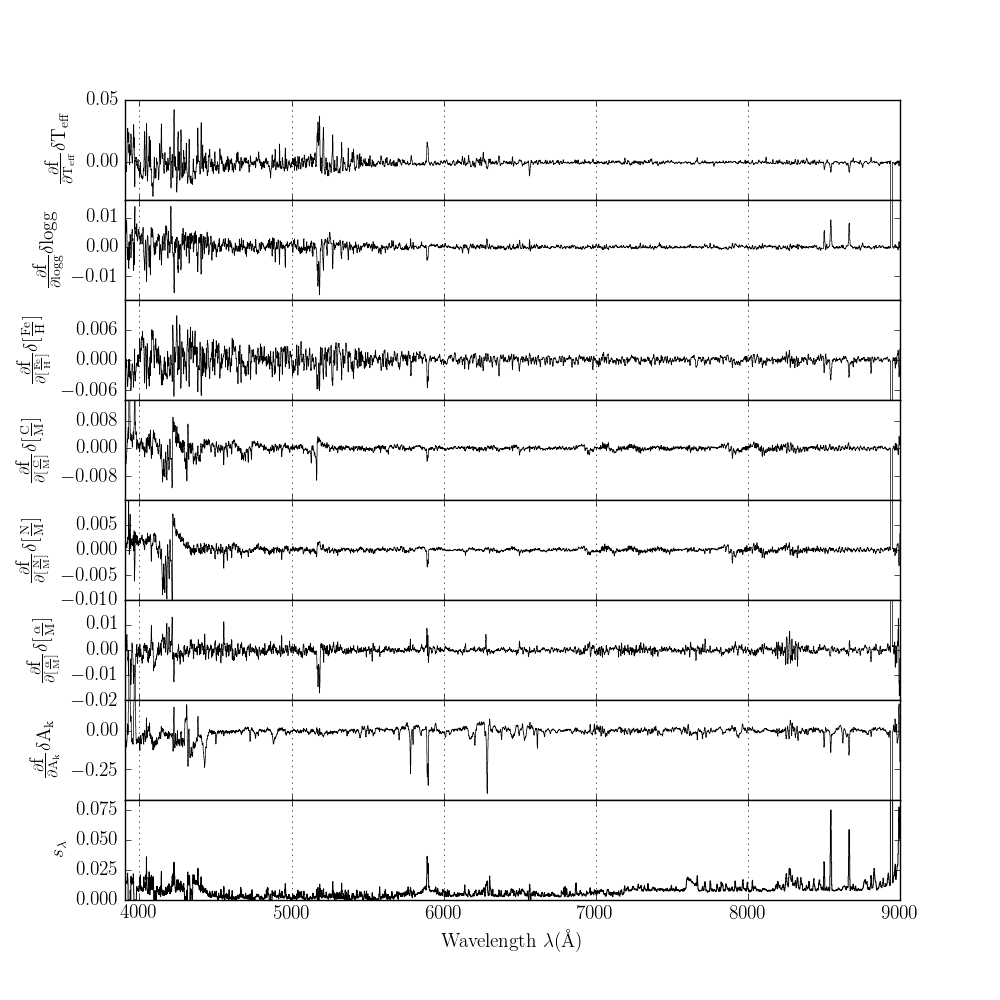
\includegraphics[scale=0.7]{leading_coeffs.png}
\caption{Leading (linear) coefficients and scatter 
  from the best-fit spectral model, 
determined by \tc\ using the \ntrobj\ reference objects. 
These leading coefficients indicate how sensitive each pixel 
in the spectrum is to each of the labels. 
Scaled by the approximate errors in the labels:
91.5~K in \teff, 0.11 in \logg, 0.05 for \mh, \alpham, and \carbon, 
and 0.06 for \nitrogen. 
\Comment{AYQH}{Not sure about uncertainties in C and N...}
\citep{Holtzman2015}.}
\label{fig:leading-coeffs}
\end{figure}

We can compare Figure \ref{fig:leading-coeffs} to 
theoretical models for what the sensitivity to
\carbon\ and \nitrogen\ should be
at these wavelengths. Figure \ref{fig:model-cn}
shows G-band indices for \nfe\ and \cfe\ from
3800\, to 4400\, \angstrom. Figure \ref{fig:cannon-cn}
shows the corresponding region of our spectral model.
It is gratifying that the peaks in the leading coefficients
for \carbon\ and \nitrogen\ correspond to the regions
of highest sensitivity in the model: 4100-4200\,\angstrom\ 
for both elements, with a feature at 4300\,\angstrom\ for 
\carbon. 

\begin{figure}[!p]
\centering
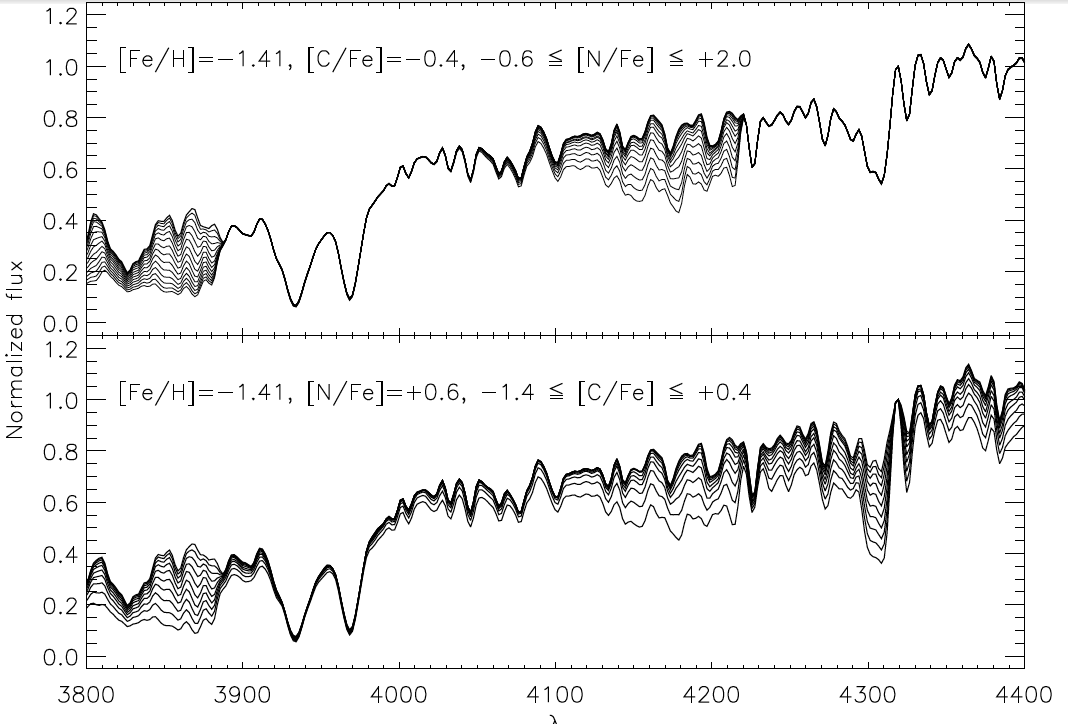
\includegraphics[scale=0.4]{model_c_n.png}
\caption{
Figure taken from \citet{Martell2008}. In both the 
top and bottom panel, the thick black line is
a synthetic spectrum. The overlaid thin lines are
the G-band indices for \cfe\ (top panel) and
\nfe\ (bottom panel). In other words, thicker
regions of the spectrum correspond to regions that
are predicted by theoretical models to be more 
sensitive to \cfe\ and \nfe\ (top and bottom panel, respectively). 
}
\label{fig:model-cn}
\end{figure}

\begin{figure}[!p]
\centering
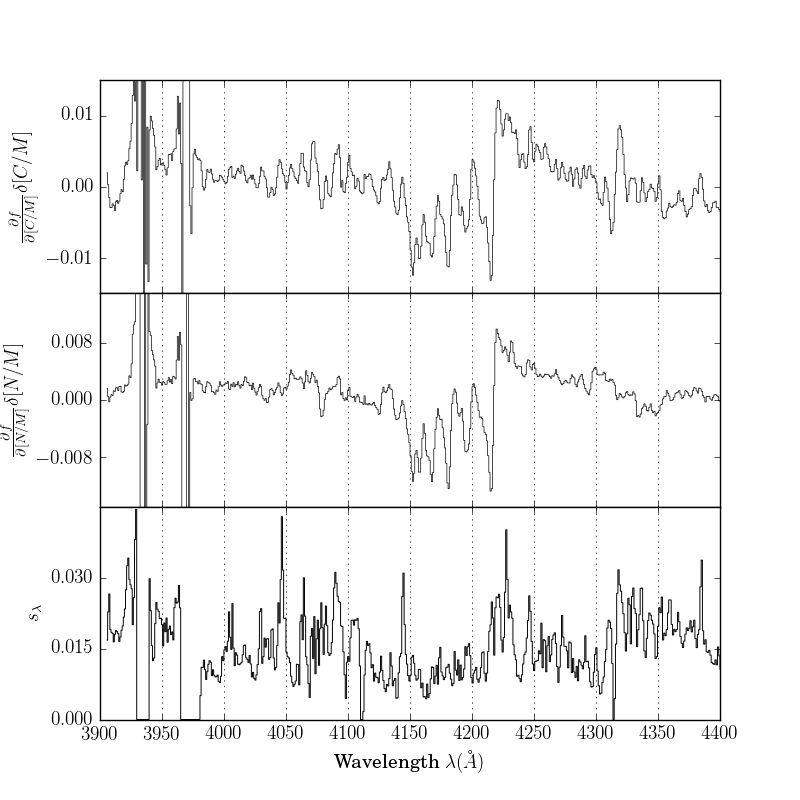
\includegraphics[scale=0.8]{leading_coeffs_ages_zoom.png}
\caption{
A zoom-in of Figure \ref{fig:leading-coeffs} for 
\carbon\ and \nitrogen, 
for a direct comparison to Figure \ref{fig:model-cn}.
It is gratifying to see that both the theoretical model and the data-driven Cannon
model find sensitivity to these two elements
in the 4100-4200\,\angstrom\ region. 
}
\label{fig:cannon-cn}
\end{figure}

\section{Cross Validation}

To test the model, we use it to infer new labels for the
\ntrobj\ reference objects, and compare the results 
to the original \apogee\ labels used in training.
Figure \ref{fig:cross-validation} and 
shows the results of
this cross-validation test. The very low bias
and scatter values demonstrate 
that the model has successfully
captured information about these seven labels in the
\lamost\ spectra.

\begin{figure}[!hp]
\centering
\includegraphics[scale=0.75]{xval_5panel.png}
\caption{Cross-validation of \tc 's label transfer from \apogee\ to \lamost~: Shown are the \apogee\ labels of all reference objects compared to the labels derived from \lamost\ data by \tc\ in the test step. This is a take-none-out test. The tight one-to-one correlations in the \teff , \logg~ \feh, and \alpham\ panels simply reflect the quality of the label transfer demonstrated in \citet{Ho2016}.
We include extinction as a panel
but emphasize that ours is not a reliable method for 
inferring extinction from \lamost\ spectra.
The scatter and bias values represent spectra with \snr\textgreater\,50.
}
\label{fig:cross-validation}
\end{figure}

We can independently measure mass using the standard seismic scaling relation (e.g. Kjeldsen \& Bedding 1995):

\begin{equation} \label{eq:mass}
M= \left( \frac{\nu_{\mathrm{max}}}{\nu_{\mathrm{max,\odot}}}\right)^3\  \left( \frac{\Delta \nu}{\Delta \nu_{\odot}}\right)^{-4} \ \left( \frac{T_{\mathrm{eff}}}{T_{\mathrm{eff,\odot}}}\right)^{1.5} \ 
\end{equation}





\section{Test Step}
\label{test-step}

Finally, we use our inferred \carbon\ and \nitrogen\ 
labels together with the formula in \citet{Martig2016}
to calculate ages for \ntestobj\ \lamost\ objects not observed by \apogee.

To choose which objects to apply the formula to,
we apply the same cuts as in \citet{Martig2016}:
$\mh > -0.8$, $4000 < \teff < 5000$, $1.8 < \logg < 3.3$,
$-0.25 < \cm < 0.15$, $-0.1 < \nm < 0.45$, $-0.1 < [(C+N)/M] < 0.15$,
$-0.6 < \cn < 0.2$. 

The results are shown in Figures \ref{fig:feh-alpha-logg}
and \ref{fig:feh-alpha}. 
Figure \ref{fig:feh-alpha-logg} shows the results
for all stars with a \logg\ cut applied to ensure that they
are post dredge-up giants (as per \citet{Martig2016})
and Figure \ref{fig:feh-alpha} shows the results with
a more conservative cut, to ensure that the objects
fall within the label space of the \apokasc\ reference set
used to make the model \citep{Martig2016}. 

\begin{figure}[ht!]
\centering
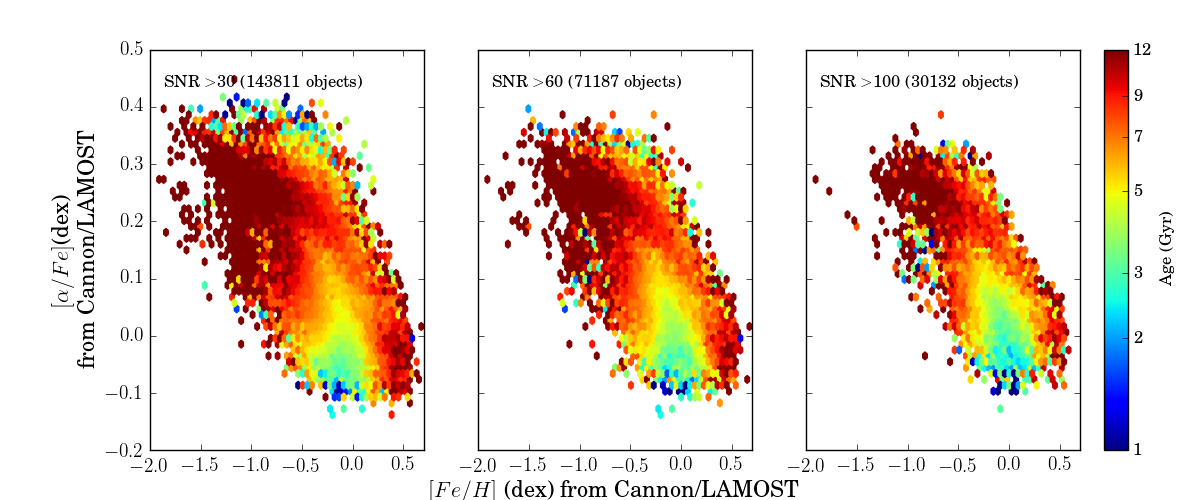
\includegraphics[scale=0.5]{feh_alpha_logg_all.png}
\caption{
The \alpham-\feh\ plane, color-coded by age, 
for \ntestobj\ objects. The \alpham\ and \feh\ values
were determined by \tc\ directly from \lamost\ spectra,
and the age values were determined using the formula
in \citet{Martig2016} and values of \carbon\ and \nitrogen\ 
determined directly from \lamost\ spectra.
}
\label{fig:feh-alpha-logg}
\end{figure}

\begin{figure}[ht!]
\centering
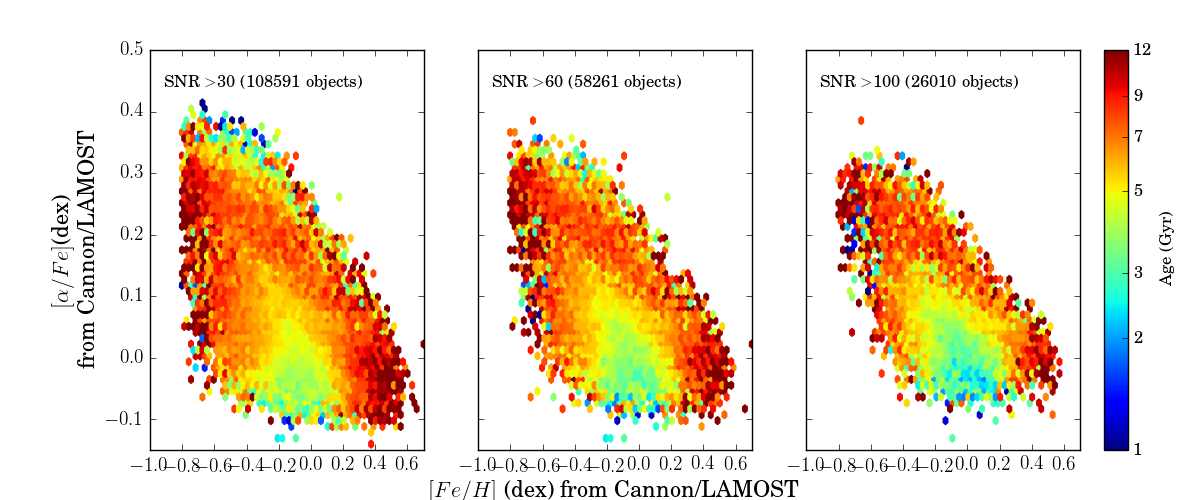
\includegraphics[scale=0.5]{feh_alpha_all.png}
\caption{
The \alpham-\feh\ plane, color-coded by age, 
for \ntestobj\ objects. The \alpham\ and \feh\ values
were determined by \tc\ directly from \lamost\ spectra,
and the age values were determined using the formula
in \citet{Martig2016} and values of \carbon\ and \nitrogen\ 
determined directly from \lamost\ spectra.
Objects outside the \apokasc\ reference set
have been cut out, as per \citet{Martig2016}.
}
\label{fig:feh-alpha}
\end{figure}

% \section{Discussion}

% At face value, we have ages to 0.25\,dex using C\&N or 
% training directly on ages. We have shown that the
% leading coefficients of C and N are very plausible,
% using gradient spectra (Yuan-Sen?) and line lists (Evan?).
% We turn C and N into ages and checked the consistency
% with the ages resulting from training directly on the 
% Kepler values. We have also verified the 
% astrophysical plausibility of the results by showing the
% distribution in the \alpham\ and \mh\ plane. 

% With this new set of ages, we have a very different
% spatial sampling than \apogee: we have essentially
% tied in-the-disk and off-the-disk ages onto the same
% scale. \lamost\ has a much better sampling of the thick
% disk than \apogee. Perhaps we can even try more labels
% in the future...

\begin{thebibliography}{24}
\expandafter\ifx\csname natexlab\endcsname\relax\def\natexlab#1{#1}\fi

\bibitem[Bovy et al.(2015)]{Bovy2015} Bovy, J., Rix, H.-W., 
Schlafly, E.~F., et al.\ 2015, arXiv:1509.05796 

\bibitem[Ho et al.(2016)]{Ho2016} Ho, A.~Y.~Q., Ness, M.~K., 
Hogg, D.~W., et al.\ 2016, arXiv:1602.00303 

\bibitem[Holtzman et al.(2015)]{Holtzman2015} Holtzman, J.~A., 
Shetrone, M., Johnson, J.~A., et al.\ 2015, arXiv:1501.04110 

\bibitem[Luo A.L., Bai Z.R. et al.(2015)]{Luo2015} Luo, A.L., Bai, Z.~R., et al.\ 2015, RAA, in press

\bibitem[Martell et al.(2008)]{Martell2008} Martell, S.~L., Smith, 
G.~H., \& Briley, M.~M.\ 2008, \pasp, 120, 839 

\bibitem[Martig et al.(2016)]{Martig2016} Martig, M., Fouesneau, M., Rix, H.-W., et al.\ 2015, arXiv:1511.08203 

\bibitem[Ness et al.(2015)]{Ness2015} Ness, M., Hogg, D.~W., 
Rix, H.-W., Ho, A.~Y.~Q., \& Zasowski, G.\ 2015, \apj, 808, 16 

\bibitem[Ness et al.(2016)]{Ness2016} Ness, M., Hogg, D.~W., 
Rix, H., et al.\ 2016, arXiv:1511.08204 

\bibitem[Rix 
\& Bovy(2013)]{RixBovy2013} Rix, H.-W., \& Bovy, J.\ 2013, \aapr, 21, 61 

\bibitem[Soderblom(2010)]{Soderblom2010} Soderblom, D.~R.\ 2010, \araa, 48, 581 

\bibitem[Soderblom(2015)]{Soderblom2015} Soderblom, D.~R.\ 2015, 
Astrophysics and Space Science Proceedings, 39, 3 

\bibitem[Wu et al.(2011)]{Wu2011} Wu, Y., Luo, A.-L., Li, 
H.-N., et al.\ 2011, Research in Astronomy and Astrophysics, 11, 924 

\end{thebibliography}

\end{document}
